\chapter{Les modèles de rendements financiers}

\section{L'utilisation de modèles en finance}
\label{sec:utilisationmodeles}

On doit considérer les implications de l'utilisation de modèles en
finance avant d'entreprendre leur étude. On doit aussi prendre
connaissance des différents types ainsi que les risques liés à chacun
d'entre eux. Pour ce faire, on se réfère à la note «Model Risk»
publiée par \cite{derman1996modelrisk}.

Durant les dernières décennies, plusieurs modèles sont apparus afin de
fournir une approche fondamentale aux concepts de tarification,
d'offre et de demande et d'arbitrage aux intervenants des milieux
financiers. Au cours des années 1970, on se préoccupe particulièrement
des fluctuations des taux d'intérêt, un phénomène qui marque cette
époque. Les notions de duration et de convexité font alors leurs
débuts. Sur les marchés de capitaux propres, on s'intéresse à la
discordance entre le prix négocié des contrats à terme et le prix
raisonnable calculé selon une perspective théorique.

Puis, la confiance développée envers le modèle de tarification
d'options de \cite{black1973pricing} et ses extensions a favorisé la
croissance du marché des produits dérivés. La puissance de calcul
croissante des ordinateurs a aussi permis l'élaboration et
l'utilisation de modèles de plus en plus sophistiqués. La dépendance
qui peut se développer envers ceux-ci apporte son lot de
considérations. On doit donc se rappeler l'utilisation désirée par les
auteurs de ceux-ci et le risque associé à leur usage à grande échelle.

\subsection{Différents types de modèles}
\label{sec:differentsmodeles}

Toujours selon Derman, un modèle financier peut être classé parmi au
moins trois catégories:

\begin{enumerate}
\item Le \textbf{modèle fondamental}, basé sur un système de postulats
  et de données, entre lesquels on peut établir différentes
  relations. Le modèle de Black-Scholes en est un exemple.
\item Le \textbf{modèle phénoménologique}, qui présente une
  description ou une analogie, afin d'illustrer quelque chose qui ne
  peut être directement observé. C'est un modèle moins fondamental,
  basé aussi sur des liens de cause à effet. Un modèle qui chercherait
  à expliquer l'impact du retrait du porteur de parts majoritaire
  d'une entreprise sur la valeur des actions de celle-ci serait
  phénoménologique.
\item Le \textbf{modèle statistique}, basé sur une régression ou un
  réglage optimal entre différents ensembles de données. On ne cherche
  pas ici à expliquer une dynamique, mais à décrire une tendance ou
  une corrélation. Le modèle d'évaluation des actifs financiers et
  celui des trois facteurs de \cite{fama1993common} en sont des exemples.
\end{enumerate}

Un modèle financier est en partie basé sur des variables qui
représentent des opinions et des anticipations, et non seulement des
quantités mesurables. Ces variables peuvent être, entre autres, le
rendement et la volatilité future espérés. Cette considération sera
importante notamment lorsque l'on voudra déterminer le prix
raisonnable d'un produit dérivé. En effet, un modèle de tarification
est essentiellement un moyen de refléter l'intuition des acteurs du
marché à propos de ces variables sous la forme d'un prix exprimé dans
une unité monétaire. Un bon modèle doit faciliter l'extrapolation de
ce prix sous certaines conditions de marché.

Contrairement à la physique classique, un principe fondamental en
finance est l'incertitude. On ne peut anticiper la valeur d'un titre à
un moment donné dans le futur avec la même précision qu'on peut
prévoir la position d'un objet à cet instant. Les outils mathématiques
principalement utilisés seront alors les processus stochastiques, les
statistiques et les distributions de probabilités, en plus du calcul
différentiel et intégral.

\subsection{Le risque de modélisation}
\label{sec:modelerisque}

Plusieurs risques inhérents à la modélisation en finance
existent. Quelques-uns d'entre eux seront décrits dans cette section.

La modélisation peut tout simplement ne pas être applicable à la
situation étudiée. L'exemple le plus probant serait de tenter de
prévoir les mouvements du prix d'un titre financier à court terme.

Un modèle peut être incorrect pour plusieurs raisons. Entre autres, il
peut ignorer certains facteurs ou poser une hypothèse déterministe
inappropriée sur ceux-ci. Il peut aussi considérer une dynamique
incorrecte pour un des facteurs ou encore une relation inappropriée
entre ceux-ci. Enfin, il peut n'être applicable que sous certaines
conditions bien précises ou encore que son utilisation soit limitée à
court terme, notamment lorsqu'il nécessite un temps de calibration
pour être statistiquement valable. Il peut aussi être inutilisable par
une mauvaise estimation des paramètres.

Un modèle peut aussi être correct, mais avoir une solution
erronée. Cela se produit notamment lorsqu'on tente de dériver une
solution analytique ou que l'on doit utiliser des méthodes numériques
pour obtenir celle-ci. On se doit, dans ce cas, de connaître l'erreur
maximale possible de la méthode utilisée. Un modèle correct peut aussi
être utilisé dans le mauvais contexte. Par exemple, on pourrait avoir
recours à des paramètres inadéquats de simulation, ou encore réutiliser le
modèle dans une autre situation sans tenir compte des
conditions de validité de celui-ci.

Son utilisation peut génèrer des prix déraisonnables; on parle alors
d'arbitrage de modèle. Par exemple, si un titre est évalué à l'aide du
modèle d'évaluation des actifs financiers, son prix sera différent de
celui qui serait obtenu avec la régression à trois facteurs de Fama et
French. Un investisseur peut alors faire du profit en achetant le
titre à celui qui demande le prix le plus faible pour le revendre à
celui qui offre le plus élevé.

L'utilisation de données instables peut produire des résultats
différents selon la période étudiée. La possibilité qu'une estimation
basée sur des données historiques soit erronée doit être considérée.

Enfin, comme la plupart des modèles financiers sont implémentés sous
forme de logiciels, différents bogues informatiques peuvent se
retrouver dans le code source. On considère entre autres des erreurs
d'arrondissement, de logique et de clarté du code, ainsi que des
particularités du matériel qui n'auraient pas été prises en compte par
le programmeur. Ces erreurs peuvent être difficiles à détecter, c'est
pourquoi un grand nombre de tests devraient être effectués avant de
publier un logiciel de modélisation financière.

\section{Les rendements financiers}
\label{sec:prixrendements}

Le \textbf{rendement} est défini comme étant le gain ou la perte de
valeur d'un actif sur une période donnée. Il est constitué des revenus
occasionnés et des gains en capitaux d'un investissement et est
habituellement représenté sous la forme d'un pourcentage. Ces derniers
peuvent prendre la forme de coupons pour les titres à revenus fixes et
de dividendes pour les actions échangées sur les marchés boursiers. On
ne considèrera, dans ce texte, que les titres boursiers sans
dividende, dont le rendement est lié uniquement aux gains en capitaux.

\subsection{Définitions et notations}
\label{sec:defrendements}

On définit le prix $S(t)>0$ d'un titre financier observé au temps
$t$. Implicitement, le prix considéré est celui à la fermeture. On
définit aussi le taux de rendement effectif $R(t)$ sur une période
comprise dans l'intervalle de temps $\left[t-1,t\right]$.  C'est le
taux composé continument, aussi appelé force d'intérêt, qui aurait
occasionné les mêmes gains ou pertes sur un montant déposé en banque
au cours de la période concernée. Le taux de rendement est la variable
d'intérêt dans le contexte de la modélisation financière.

On associe le taux de rendement effectif à la différence entre le
logarithme du prix initial et final. Dans la situation où le taux de
rendement est déterministe et non aléatoire, on obtient l'équation
différentielle suivante:
\begin{align*}
  \frac{dS(t)}{dt} &= R(t) \cdot S(t).
\end{align*}

On peut interpréter cette équation en affirmant que la variation du
prix $dS(t)$ sur un intervalle de temps infiniment petit $dt$ est
proportionnelle à la valeur actuelle $S(t)$. Cette équation
différentielle a pour solution générale:
\begin{align}
  \label{eq:solutiondiffrendement}
  S(t) &= S(0)e^{R(t) \cdot t}.
\end{align}

Afin de définir les propriétés de l'échantillon sélectionné, on pose
comme hypothèse:
\begin{hypothese}
  Le rendement $R(t)$ est constant durant la période définie par
  l'intervalle de temps $\left[t-1,t\right]$, mais il est différent
  d'une à l'autre: $R(s) \neq R(t), s \neq t$.
\end{hypothese}

On peut alors représenter le rendement $R(t)$ comme étant la
différence entre les logarithmes des prix observés au temps $t$ et
$t-1$, ou encore le logarithme du quotient de ces mêmes prix:
\begin{align}
  R(t) &= \ln{(S(t))} - \ln{(S(t-1))} \nonumber\\
  &=
  \ln{\left(\frac{S(t)}{S(t-1)}\right)}. \label{eq:rendementlogprix}
\end{align}

On définit aussi le \textbf{rendement cumulé} $L(t)$. Il correspond à
la somme des rendements effectifs observés sur l'intervalle
$\left[0,t\right]$:
\begin{align}
  L(t) &= \sum_{i=1}^{t} R(i) \nonumber\\
  &= \sum_{i=1}^{t} \left[\ln{(S(i)} - \ln{(S(i-1))}\right] \nonumber\\
  &= \ln{(S(t))} - \ln{(S(0))} \nonumber\\
  &= \ln{\left(\frac{S(t)}{S(0)}\right)}. \label{eq:rendementcumL}
\end{align}

Cette représentation permet d'exprimer le prix actuel $S(t)$ en
fonction de la valeur initiale $S(0)$ sous une forme similaire à la
solution \eqref{eq:solutiondiffrendement}, mais tenant compte de
l'hypothèse émise précédemment:
\begin{align}
  e^{L(t)} &= \frac{S(t)}{S(0)} \nonumber\\
  S(t) &= S(0) \cdot e^{L(t)} \nonumber\\
  &= S(0) \cdot \exp\left(\sum_{i=1}^{t} R(i)\right).
\end{align}

\subsection{Rendements cumulés}
\label{sec:rendementscum}

On pose l'hypothèse suivante:
\begin{hypothese}
  Les rendements $R(i), i \in 1, \ldots, t$ sont indépendants, mais
  pas nécessairement identiquement distribués.
\end{hypothese}

On peut alors obtenir la distribution du rendement cumulé $L(t)$ en
utilisant le produit de convolution \eqref{eq:convocaract}.
Considérons $\phi_{R(i)}(\xi)$ la fonction caractéristique d'un
rendement $R(i)$ et $\phi_{L(t)}(\xi)$ celle du cumulé $L(t)$. On
obtient alors que cette dernière est égale au produit des fonctions
caractéristiques des rendements effectifs sur chacune des périodes de
l'intervalle $\left[0,t\right]$:
\begin{equation}
  \label{eq:convolutionLR}
  \phi_{L(t)}(\xi) = \prod_{i=1}^t  \phi_{R(i)}(\xi).
\end{equation}

On considère la situation où l'on posera plutôt l'hypothèse suivante:
\begin{hypothese}
  Les rendements $R(i), i \in 1, \ldots, t$ sont à la fois
  indépendants et identiquement distribués.
\end{hypothese}

Alors, la fonction caractéristique des rendements est égale pour
chaque période:
\begin{align}
  \label{eq:rendementsIID}
  \phi_{R}(\xi) = \phi_{R(1)}(\xi) = \ldots &= \phi_{R(t)}(\xi).
\end{align}

On peut donc simplifier l'expression \eqref{eq:convolutionLR} pour
obtenir la fonction caractéristique:
\begin{equation}
  \label{eq:convolution2}
  \phi_{L(t)}(\xi) = \left[\phi_{R}(\xi)\right]^t.
\end{equation}

Considérer une distribution qui est fermée sous la convolution pour
modéliser les rendements sur une période $R(i)$ peut alors être
intéressant. Le rendement cumulé $L(t)$ pourra aussi être
modélisé à l'aide de la même distribution. Pour ce faire, on modifie
un paramètre d’échelle en fonction de la longueur $t$ de l'intervalle
de temps considéré.

\subsection{Données disponibles}
\label{sec:donneesdisponibles}

Les données disponibles auprès des fournisseurs d'informations
financières prennent habituellement la forme de séries chronologiques
discontinues. Celles-ci incluent les prix à l'ouverture, le plus bas
et le plus élevé au courant de la journée ainsi qu'à la fermeture,
pour chaque jour où les marchés financiers sont en activité. Afin de
mesurer le rendement quotidien d'un titre, seuls les prix à la
fermeture seront considérés.

\section{Les premiers modèles}

\subsection{Le modèle de Bachelier}
\label{sec:bachelier}

Un des premiers modèles proposés afin de représenter les rendements
financiers a été celui de \cite{bachelier1900theorie} .

Le prix d'un titre peut varier, durant une période, de n'importe
quelle valeur comprise dans l'intervalle $\left[ -S(t),\infty
\right]$. Il propose donc que cet intervalle soit remplacé par
l'ensemble du domaine réel $\mathbb{R}$. La probabilité que le titre
atteigne une valeur nulle ou négative ou que celle-ci double devrait
donc être négligeable. Il ajoute aussi que la variation est
indépendante du prix actuel du titre $S(t)$ et que la distribution de
probabilités de celle-ci est symétrique et centrée en ce point.

Il utilise le principe selon lequel la probabilité que deux évènements
indépendants consécutifs aient lieu est le produit de celles que
chacun d'entre eux se réalise, pour établir la distribution des
variations du prix. Par exemple, la variation du prix sur une première
période prend la valeur $x$ et celle sur une seconde, $z-x$, comme
illustré à la figure \ref{fig:bachelier1}.

%% ligne du temps
\begin{figure}[!ht]
  \centering
  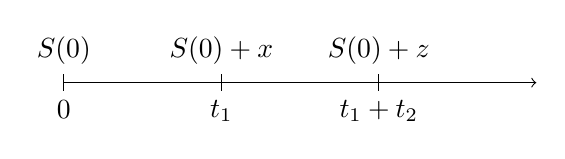
\begin{tikzpicture}
    \draw [->] (0,0) -- (6,0); \foreach \x in {0,2,4} \draw (\x
    cm,3pt) -- (\x cm,-3pt); \draw (0,0) node[below=3pt] {$ 0 $}
    node[above=3pt] {$ S(0) $}; \draw (2,0) node[below=3pt] {$ t_1 $}
    node[above=3pt] {$ S(0)+x $}; \draw (4,0) node[below=3pt] {$
      t_1+t_2 $} node[above=3pt] {$ S(0)+z $};
  \end{tikzpicture}
  \caption{Modèle de Bachelier: probabilité composée}
  \label{fig:bachelier1}
\end{figure}

On définit $f(x,t)$ la fonction de densité de la variation du prix
$S(t)$ par rapport au niveau initial $S(0)$. Alors, selon le principe
précédent, on obtient l'expression
\begin{align}
  \label{eq:probcomposeeB}
  f(z,t_1+t_2) = \int_{-\infty}^{\infty} f(x,t_1)\cdot f(z-x,t_2)
  \cdot dx.
\end{align}

La solution proposée est que la densité de probabilité soit de la forme
\begin{align*}
  \label{eq:formeprobB}
  f(x,t) = A \cdot \exp \left\{-B^2x^2 \right\}.
\end{align*}

Afin que la fonction $f(x,t)$ soit une densité de probabilité, la
condition suivante doit être respectée:
\begin{align}
  \int_{-\infty}^{\infty} A \cdot \exp \left\{-B^2x^2 \right\} dx = 1.
\end{align}

Ceci implique que 
\begin{align*}
  B&= A\sqrt{\pi}.
\end{align*}

En posant $x=0$, on a $A=f(0,t)$ et l'on en déduit:
\begin{align}
  f(x,t) = f(0,t) \cdot \exp \left\{-\pi \cdot f(0,t)^2 \cdot x^2
  \right\}.
\end{align}

En reprenant l'intégrale \eqref{eq:probcomposeeB}, on obtient que la
densité de probabilité $f(z,t_1+t_2)$ soit aussi de la forme
\eqref{eq:formeprobB}:
\begin{align}
  f(z,t_1+t_2) = \frac{f(x,1)f(z-x,2)}{\sqrt{f(x,1)^2+f(z-x,2)^2}}
  \exp \left\{-\pi \frac{f(x,1)f(z-x,2)}{f(x,1)^2+f(z-x,2)^2} z^2
  \right\}.
\end{align}

On reconnaitra que cette densité est, à un changement de variable
près, une loi normale. La démarche suggère qu'il recherchait une
distribution qui était fermée sous la convolution, une propriété
souhaitable pour un modèle cohérent des rendements financiers.

Ce modèle implique un processus de Wiener-Bachelier selon lequel les
incréments, ou les changements de prix, suivent une distribution
normale:
\begin{equation}
  \label{eq:bachelier00}
  S(T)-S(t) \sim N\left(0,\sigma^2 \left(T-t\right)\right).
\end{equation}

On doit noter que ce modèle implique que la variance des fluctuations
n'est pas proportionnelle au prix initial. Une première correction
sera apportée au modèle afin de considérer le logarithme du prix. Ce
changement permettra d'obtenir un modèle où elle est désormais
proportionnelle au prix initial. Le processus du prix suivra alors un
mouvement brownien géométrique:
\begin{align}
  \label{eq:browniengeom}
  S(T)-S(t) &\sim LN \left(0, \sigma (T-t) \right).
\end{align}

Le logarithme du prix suivra alors un processus de Wiener-Bachelier:
\begin{align}
  \label{eq:bachelierwiener2}
  \ln\left(S(T)\right)-\ln\left(S(t)\right) &\sim N\left(0,\sigma
    \left(T-t\right)\right).
\end{align}

Un des principaux avantages du processus de Bachelier modifié est que
le rendement cumulé $L(t)$ est aussi une variable aléatoire
gaussienne. Cette propriété est appelée L-stabilité ou invariance sous
l'addition. La distribution gaussienne est la seule ayant cette
propriété où le second moment est fini. Le sujet des distributions L
stables sera aussi abordé à la section \ref{sec:mandelbrot}.

Quelques années après sa publication, ce modèle est l'objet de
critiques de la part d'économistes et de financiers. En se référant à
\cite{mitchell1916critique}, on observe que, sur une base annuelle,
les variations négatives par rapport à la moyenne (149) sont plus
fréquentes que celles qui sont positives (126), pour un ensemble de 40
titres boursiers, entre 1890 et 1915 (figure \ref{fig:mitchell1}).
Une asymétrie négative des rendements sera alors présente.
\begin{figure}[!ht]
  \centering
  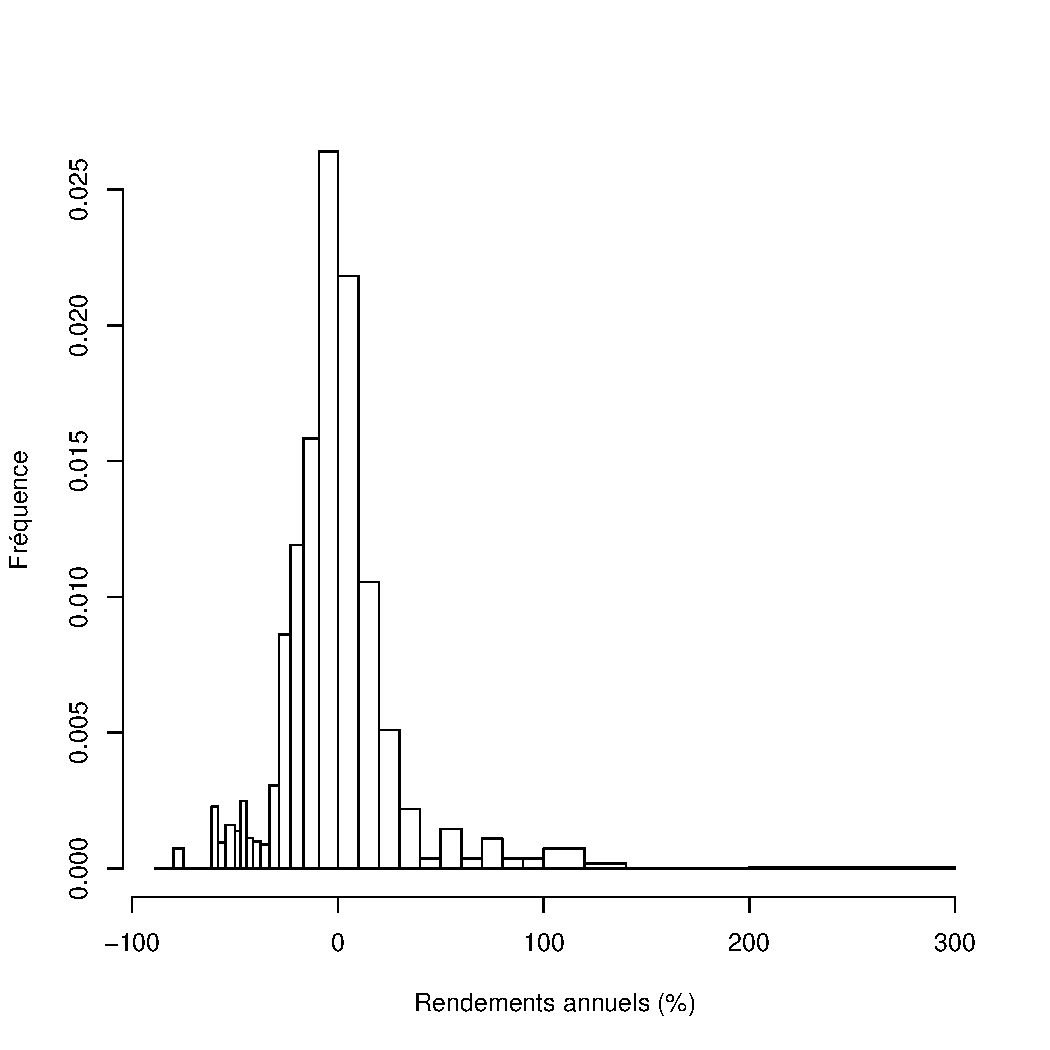
\includegraphics[scale=0.75]{./graphiques/mitchell1.pdf}
  \caption{Distribution des rendements annuels de 40 titres boursiers,
    de 1890 à 1915, Table XVIII de \cite{mitchell1916critique}}
  \label{fig:mitchell1}
\end{figure}

De plus, les variations extrêmes sont plus fréquentes que ne pourrait
le prédire un modèle basé sur un mouvement brownien. La distribution
des rendements aurait donc des queues plus épaisses
\footnote{traduction de l'anglais heavy tailed} que la normale. On
doit trouver un modèle qui permet de tenir compte de ces
particularités.

\subsection{Proposition de Mandelbrot}
\label{sec:mandelbrot}


\cite{mandelbrot1963variation} propose un modèle qui vise à combler
les lacunes du processus brownien géométrique
\eqref{eq:browniengeom}. Il explique que les distributions empiriques
des changements de prix sont habituellement trop \emph{pointues} pour
être considérées comme des échantillons d'une population gaussienne.

Il identifie différentes caractéristiques qu'un bon modèle des
rendements financiers devrait posséder:

\begin{enumerate}
  \label{enum:mandelbrot}
\item Il doit tenir compte de la fréquence des grands changements de
  prix. Il doit donc être basé sur une distribution leptocurtique,
  plus pointue au centre que la normale.
\item Il doit permettre des changements instantanés et imprévisibles
  de toute amplitude.
\item Il doit admettre une probabilité non nulle que plusieurs
  changements consécutifs semblent corrélés.
\item Il doit admettre un processus de prix non stationnaire, car la
  variance échantillonnale prend différentes valeurs à travers le
  temps.
\end{enumerate}

La famille de distributions L stables semble être celle qui répond le
mieux à l'ensemble de ces conditions \citep{walterlevy}. L'équation
suivante définit la propriété de L-stabilité de la distribution de la
variable aléatoire des rendements sur une période $R$:
\begin{align}
  (a_1 R_1 + b_1) + (a_2 R_2 + b_2) &\stackrel{d}{=} aR + b \\
  \forall a_1,a_2 > 0, \forall b_1, b_2.
\end{align}

La solution générale de cette équation a été découverte par Lévy en
1925. Le logarithme de la fonction caractéristique de celle-ci prend
la forme suivante:
\begin{align}
  \ln{(\phi_{R}(\xi))} = i\delta \xi - \gamma |\xi|^{\alpha}
  \left[1+\frac{i\beta \xi}{|\xi|} \tan{\frac{\alpha\pi}{2}} \right].
\end{align}

Le domaine et le rôle des paramètres de la distribution L stable sont
décrits à la table \ref{tab:roleparam}. La flexibilité apportée par les
quatre paramètres permet de remplir les quatre conditions établies au
début de cette section. De plus, l'absence, dans la majorité des cas,
de moments finis d'ordre supérieur à l'espérance permet de tenir
compte du mouvement erratique des prix et ainsi produire de larges
discontinuités de son processus. Elle permet aussi d'expliquer
l'apparence de corrélation sérielle, en considérant une probabilité
non négligeable que cette caractéristique soit présente. Cependant, ce
modèle est difficile à appliquer à l'évaluation de produits dérivés
pour cette raison, étant donné que l'on devra être en mesure de
quantifier la volatilité.
\begin{table}[!ht]
  \centering
  \begin{tabular}{|c|p{1.75cm}|p{2.5cm}|p{6.25cm}|}
    \hline
    \textbf{Paramètre} & \textbf{Domaine} & \textbf{Rôle} & \textbf{Observations} \\
    \hline
    $\alpha$ & $\left]0,2\right]$ & Aplatissement & Plus sa valeur est petite, plus la distribution est leptocurtique. $\alpha=2$ correspond à la distribution normale. \\
    $\beta$ & $\left] -1, 1 \right]$ & Asymétrie & Défini seulement lorsque $\alpha \neq 1$. Lorsque $\alpha=1$ et $\beta=0$, on obtient la distribution de Cauchy.  \\
    $\gamma = s^{\alpha}$ & $\mathbb{R}\setminus\{0 \}$ & Échelle & On doit prendre la racine $\alpha$ pour obtenir un paramètre d'échelle $s$ tel que défini par Pearson. \\
    $\delta$ & $\mathbb{R}$ & Localisation & \\
    \hline
  \end{tabular}
  \caption{Domaine et rôle des paramètres de la distribution L stable de Mandelbrot}
  \label{tab:roleparam}
\end{table}

L'approche classique, selon Mandelbrot, pour expliquer les grands
changements de prix a été de considérer un mélange de deux
distributions normales, dont une pour les fluctuations régulières et
une qui a une variance plus importante, pour les discontinuités. Il
remarque que pour expliquer adéquatement le comportement des données
empiriques, on doit introduire un mélange de plusieurs distributions
normales, ce qui rendrait le modèle plus complexe. Par contre, on
retrouve une approche intéressante avec le modèle présenté à la
section suivante.

\subsection{Le modèle de Press}
\label{sec:press}

\cite{press1967compound} propose un modèle statistique basé sur un
processus de Poisson composé auquel on ajoute un mouvement brownien
$W(t)$. C'est donc d'un processus ayant des incréments stationnaires
et indépendants. Il présente donc les caractéristiques d'un processus
de Lévy. Press utilise aussi la transformation logarithmique
\eqref{eq:browniengeom} afin que la variation soit proportionnelle au
prix. Il remarque aussi que le modèle logarithmique de Bachelier est
inadéquat, car il ne tient pas compte des queues de la distribution
empirique des rendements qui sont plus épaisses que celles de la
normale. Il ajoute que le modèle proposé par Mandelbrot est
discutable, car il ne trouve aucune évidence, à partir des données
observées, que la distribution de la population aurait une variance
infinie.

Le processus de Poisson $\left\{N(t)\right\}$ de paramètre $\lambda t$
est un processus de comptage qui détermine les occurrences des sauts
$Y_k, k = 1, \ldots, N(t)$. Ces sauts surviennent généralement
lorsqu'une information importante est rendue publique par rapport à un
titre. Ceux-ci sont aussi de distribution normale, mais leur espérance
n'est pas nulle et leur variance est différente de celle du processus
$W(t)$. Cette composante que l'on ajoute au modèle de Bachelier
modifié permet d'expliquer les variations plus importantes et moins
fréquentes observées empiriquement.

Le processus du logarithme du prix $\left\{s(t)\right\} \equiv
\left\{\ln{(S(t))}\right\}$ est donc représenté par l'équation
suivante:
\begin{align}
  \label{eq:press67}
  s(t) &= s(0) + \sum_{k=1}^{N(t)} Y_k + W(t).
\end{align}

On définit les différentes variables aléatoires composant le processus
comme suit:
\begin{align*}
  Y_k &\sim N(\theta,\sigma_2^2) \\
  W(t) &\sim N(0,\sigma_1^2 t) \\
  N(t) &\sim Poisson(\lambda t)
\end{align*}

Comme pour la plupart des processus de Lévy, on ne peut obtenir une
forme explicite pour la fonction de densité, car celle-ci se présente
sous la forme d'une série infinie. On représente alors ces processus
par leur fonction caractéristique, formée par le produit de celles de
leurs différentes composantes.

La distribution du logarithme du prix $s(t)$ est définie par la
fonction caractéristique $\phi_{s(t)}(\xi)$, qui est le produit de
celle de la constante et celles des processus de Wiener et de Poisson
composé:
\begin{align}
  \label{eq:fncaractpress}
  \phi_{s(t)}\left(\xi\right) &= E\left[e^{i \xi s(t)} \right] \nonumber \\
  &= exp\left\{ i\xi \cdot s(0) \right\} \times exp \left\{ -\frac{t \sigma_1^2 \xi^2}{2} \right\} \times exp \left\{ \lambda t \left[e^{i \theta \xi-(\sigma_2^2 \xi^2/2)}-1 \right] \right\} \nonumber \\
  &= exp\left\{ i\xi \cdot s(0)- \frac{t}{2}\sigma_1^2\xi^2 + \lambda
    t \left[e^{i \theta \xi-(\sigma_2^2 \xi^2/2)}-1 \right] \right\}.
\end{align}

Afin d'estimer le modèle, on s'intéressera plutôt à la distribution
d'un incrément $\Delta s(t) = s(t)-s(t-1)$ de ce processus. La
fonction caractéristique $\phi_{\Delta s(t)}(\xi)$ de cette variable
aléatoire peut être facilement identifiée à partir de celle du
processus \eqref{eq:fncaractpress}. Essentiellement, on pose $s(0)=0
\mbox{ et } t=1$, pour obtenir:
\begin{align}
  \label{eq:fncaractpress2}
  \phi_{\Delta s(t)}\left(\xi\right) &= E\left[e^{i\xi\Delta s(t)} \right] \nonumber \\
  &= exp\left\{-\frac{\sigma_1^2 \xi^2}{2} + \lambda \left[e^{i
        \xi\theta -(\sigma_2^2 \xi^2/2)}-1 \right] \right\}.
\end{align}

Pour estimer les paramètres du modèle, on privilégie la méthode des
cumulants, qui est similaire à la méthode des moments. Considérons les
quatre premiers cumulants de la distribution de l'incrément $\Delta
s(t)$:
\begin{subequations}\label{eq:cumulantspress}
  \begin{align}
    K_1 &= \lambda\theta \\
    K_2 &= \sigma_1^2+\lambda(\theta^2+\sigma_2^2) \\
    K_3 &= \lambda\theta(\theta^2+3\sigma_2^2) \\
    K_4 &= \lambda(\theta^4 + 6 \theta^2 \sigma_2^2 + 3 \sigma_2^4).
  \end{align}
\end{subequations}

En utilisant les quatre premiers cumulants empiriques
\eqref{eq:cumulantsempiriques}, on obtient les équations suivantes:
\begin{subequations}\label{eq:presscum}
  \begin{align}
    0 &= \hat\theta^4 - \frac{\overline{K}_3}{\overline{K}_1} \hat\theta^2 + \frac{3\overline{K}_4}{2\overline{K}_1} \hat\theta - \frac{\overline{K}_3^2}{2\overline{K}_1^2} \label{eq:presscumtheta}\\
    \hat\lambda &= \frac{\overline{K}_1}{\hat\theta} \label{eq:presscumlambda}\\
    \hat\sigma_2^2 &= \frac{\overline{K}_3-\hat\theta^2\overline{K}_1}{3\overline{K}_1} \label{eq:presscumsigma2}\\
    \hat\sigma_1^2 &= \overline{K}_2 -
    \frac{\overline{K}_1}{\hat\theta}\left(\hat\theta^2 +
      \frac{\overline{K}_3 - \overline{K}_3 \theta^2}{3\overline{K}_1}
    \right). \label{eq:presscumsigma1}
  \end{align}
\end{subequations}

En résolvant numériquement l'équation \eqref{eq:presscumtheta} pour le
$\hat\theta$, puis par substitutions successives dans les équations
\eqref{eq:presscum}, on obtient des estimateurs convergents pour les
quatre paramètres du modèle.

Un modèle similaire a aussi été présenté par \cite{merton1976option},
cependant, il inclut un paramètre de dérive $\alpha$, et considère que
les sauts $Y$, qui sont des facteurs multiplicatifs, peuvent suivre une autre distribution que la normale. Il
présente le modèle sous la forme d'une équation différentielle
stochastique:
\begin{align}
  \label{eq:modelemerton}
  \frac{dS}{S} = (\alpha - \lambda k)dt + \sigma dW + dq.
\end{align}
La constante $k$ représente l'espérance de la variation relative si un
saut se produit et $q$, le processus de Poisson composé. La solution
de cette équation est, selon le lemme d'Itô:
\begin{align}
  S(t) &= \tilde{S}(0) \exp \left\{
    (\alpha-\frac{1}{2}\sigma^2-\lambda k)t +
    \sigma W(t) \right\}
    \end{align}
    où
    \begin{align}
  \tilde{S}(0) &= \begin{cases}
    S(0) & \text{si } N(t) = 0\\
    S(0) \sum_{k=1}^{N(t)} Y_k & \text{si } N(t) \geq 1. \nonumber
  \end{cases}
\end{align}

En spécifiant un paramètre de dérive $\delta =
\alpha-\frac{1}{2}\sigma^2-\lambda k$ et en considérant que les
sauts $Y$ sont de distribution lognormale, on peut réécrire la
fonction caractéristique d'un incrément \eqref{eq:fncaractpress2} du
modèle de Press:
\begin{align}
  \label{eq:fncaractmerton}
  \phi_{\Delta s(t)}\left(\xi\right) &= E\left[e^{i\xi\Delta s(t)} \right] \nonumber \\
  &= \exp\left\{i\delta \xi -\frac{\sigma^2 \xi^2}{2} + \lambda
    \left[e^{i \xi\theta -(\sigma^2 \xi^2/2)}-1 \right] \right\}.
\end{align}

L'utilisation de ce modèle présente deux désavantages. L'estimation du
modèle est difficile lorsque la moyenne s'approche de 0, car le
quotient \eqref{eq:presscumlambda} tend alors vers une
indétermination. De plus, contrairement à d'autres modèles, il est
difficile d'identifier le rôle des paramètres par rapport à un moment
en particulier (classification de Pearson), contrairement à ce qu'on
pourra observer avec la distribution de Laplace asymétrique
généralisée.

\subsection{Le modèle de Praetz}

\cite{praetz1972distribution} propose un modèle inspiré par la
physique des particules. Il pose comme hypothèse que deux intervalles
qui ne se chevauchent pas forment une marche aléatoire, et que les
éléments qui composent la séquence des rendements financiers $\left\{
  R(t) \right\}$ sont mutuellement indépendants. Il considère qu'un
état stable existe où les rendements suivent une loi normale de
paramètres $\mu$ et $\sigma^2$.

Cependant, cet état stable n'est jamais réellement atteint, et la
fonction de densité empirique généralement observée suppose une
distribution symétrique concave, pointue au centre et ayant des queues
épaisses. Il fait une analogie entre la température d'un gaz et le
niveau d'activité sur les marchés, où la variance du mouvement
brownien est proportionnelle à ces deux quantités. Il propose que le
paramètre de variance de la normale $\sigma^2$ suive une distribution
$g(\sigma^2)$ ayant un support positif. La distribution conditionnelle
est normale lorsque ce paramètre est connu.
\begin{align}
  h_{R(t)}(r) &= \int_0^{\infty} f_{R(t)}(r|\sigma^2) g(\sigma^2) d\sigma^2 \\
  f_{R(t)}(r|\sigma^2) &= \frac{1}{\sigma\sqrt{2\pi}}exp\left\{-\frac{(r-\mu)^2}{2\sigma^2} \right\} \label{eq:praetz72}
\end{align}

Il propose comme solution acceptable pour la densité $g(\sigma^2)$, la
distribution gamma inverse de paramètres $m$ et $s^2$:
\begin{align}
  \label{eq:gpraetz}
  g(\sigma^2) &=
  \frac{s^{2m}(m-1)^me^{-(m-1)\frac{s^2}{\sigma^2}}}{\sigma^{2(m-1)}\Gamma(m)}.
\end{align}

Cette distribution a pour moyenne $s^2$ et variance $\frac{s^2}{m-2}$.
La distribution non conditionnelle des rendements $h_{R(t)}$ est
approximativement une Student avec $2m$ degrés de liberté à un facteur
d'échelle de $\left(\frac{m}{m-1}\right)^{1/2}$ près:
\begin{align}
  \label{eq:hpraetz}
  h_{R(t)}(r) &= \frac{\Gamma(m)\left[\ 2(m-1)\pi
    \right]^{1/2}s}{\left[1+\frac{(y-\mu)^2}{s^2(2m-2)}
    \right]^{m+1/2}}.
\end{align}

D'autres distributions pourraient être utilisées au lieu de la gamma
inverse. En utilisant la loi gamma, on obtient la distribution de
Laplace asymétrique généralisée, qui sera l'objet d'une étude
approfondie aux chapitres suivants. Il propose enfin d'utiliser aussi
la distribution a priori gamma inverse pour le paramètre $\mu$. Par
contre, il remarque qu'il obtient aussi une distribution similaire à
celle de Student. Cette généralisation n'est donc pas nécessaire.

\section{Conditions essentielles de Madan et Seneta}
\label{sec:madanseneta90}

Inspirés par les travaux de Mandelbrot, Press et Praetz,
\cite{madan1990variance} présentent un ensemble de conditions
considérées essentielles dans l'élaboration d'un modèle de rendements
financiers. Ils se baseront sur celles-ci pour proposer le modèle
Variance Gamma:

\begin{enumerate}
\item La distribution des rendements $R$ doit avoir une queue
  épaisse. Ainsi, la probabilité que cette variable aléatoire ait une
  valeur supérieure à $r+t$ avec un $t$ petit, sachant qu'elle est
  supérieure à $r$, doit tendre vers 1, ce qui signifie que la
  fonction de survie converge lorsque cette quantité est grande.
  \begin{eqnarray}
    \label{eq:condmadan1}
    \lim_{r\rightarrow \infty} P\left[R > r+t | R > r \right] &=& 1 \\
    \bar{F}(r+t) &\sim& \bar{F}(r), \qquad r \rightarrow \infty \nonumber
  \end{eqnarray}
\item La distribution doit posséder des moments finis pour les $n$
  premières puissances des rendements $R$. Étant donné que l'on
  cherche à modéliser la queue de la distribution, on fixe $n=4$.
  \begin{equation}
    \label{eq:condmadan2}
    E\left[R^k\right] < \infty, \qquad k \in \lbrace 1,2,3,4 \rbrace
  \end{equation}
\item
  \begin{enumerate}
  \item Le modèle doit proposer un processus de temps continu ayant
    des accroissements stationnaires et indépendants.
  \item Les distributions des accroissements doivent appartenir à la
    même famille, quelle que soit leur longueur. Cette condition est
    essentielle afin de permettre l'échantillonnage et l'analyse des
    séries chronologiques.
  \end{enumerate}
\item Le modèle doit permettre une extension multivariée avec une
  distribution elliptique afin de conserver la validité du modèle
  d'évaluation des actifs financiers.
\end{enumerate}

Chacun des modèles présentés précédemment respecte la majorité ou
toutes ces conditions. Les résultats se retrouvent à la table
\ref{tab:condmadan}.
\begin{table}[!ht]
  \centering
  \begin{tabular}{ccccc}
    & \multicolumn{4}{c}{\textbf{Conditions}} \\
    \hline
    \textbf{Modèles}                                       & 1 & 2 & 3 & 4 \\
    \hline
    Mouvement brownien de Bachelier              &   & $\ast$ & $\ast$ & $\ast$ \\
    Distribution stable symétrique de Mandelbrot & $\ast$ & & & $\ast$ \\
    Processus de Poisson composé de Press       & $\ast$ & $\ast$ & $\ast$ & $\ast$ \\
    Mélange gaussien/inverse gamma de Praetz     & $\ast$ & $\ast$ &   & $\ast$ \\
    Modèle Variance Gamma de Madan et Seneta     & $\ast$ & $\ast$ & $\ast$ & $\ast$ \\
    \hline
  \end{tabular}
  \caption{Respect des conditions émises par Madan et Seneta pour les différents modèles présentés}
  \label{tab:condmadan}
\end{table}

On remarque que le modèle de Press remplit toutes les conditions
émises par Madan et Seneta. Cependant, ils remarqueront que ce n'est
pas un processus de sauts, car il contient aussi une composante de
diffusion (Section \ref{sec:levykhintchine}), ce qui va à l'encontre
de l'intuition derrière la continuité de la trajectoire du prix. C'est
cette dernière observation qui les incitera à proposer le modèle
Variance Gamma, qui est un processus de sauts. Ce modèle, aussi étudié
sous le nom de distribution de Laplace asymétrique généralisée par
\cite{kotz2001laplace}, a acquis beaucoup de notoriété dans le domaine
de la finance mathématique. De plus, avec le développement de
l'informatique et des méthodes numériques, on peut maintenant utiliser
de manière efficace la fonction caractéristique dans le cadre de la
calibration, des tests statistiques et de la tarification
d'options. C'est pourquoi un intérêt particulier est apporté à cette
distribution dans ce texte.

% \section{La volatilité}
% \label{sec:volatilite}

% La \textbf{volatilité} est une mesure de l'ampleur des variations du
% prix d'un actif. Elle sert à quantifier le risque lié à un
% investissement, le plus souvent sur un horizon à court terme. Elle se
% calcule le plus souvent à partir des prix des options observés sur les
% marchés, on parle alors de volatilité implicite. Comme elle n'est pas
% mesurable, cette volatilité est le reflet de l'anticipation des
% investisseurs quant aux perspectives du marché.

% Cependant, on peut toujours mesurer la volatilité historique du prix
% d'un titre à travers les rendements passés. La première étude à ce
% sujet a été faite par Black et Scholes, les auteurs du célèbre modèle
% qui porte désormais leur nom. Ils ont conclu que leur modèle
% surestimait le prix des options pour des actifs sous-jacents ayant une
% volatilité historique élevée, le contraire se produisait lorsqu'elle
% l'était peu. Leur modèle est donc utile à condition que les
% investisseurs puissent faire de bonnes prévisions
% \citep{musiela2005martingale}.

% De plus, comme il a été expliqué précédemment, les données historiques
% démontrent que la volatilité n'est pas constante avec le temps, mais
% plutôt aléatoire. Dans cette perspective, on pourrait identifier la
% distribution de la volatilité à travers le temps.
% \subsection{Mesure de la volatilité historique}
% \label{sec:mesurevolatilite}

% Afin d'obtenir un ensemble d'observations de la volatilité historique,
% on utilise une approche par fenêtre mobile. \cite{randal2004non}
% considère un estimateur de variance mobile $\hat\sigma^2(t)$, basé sur
% les rendements centrés $R(t) = Y(t)-E\left[Y(t)\right]$ de la forme
% \begin{align}
%   \hat\sigma^2(t) = \frac{1}{2r+1} \sum_{j=-r}^r R(t+j)^2, \qquad
%   t\in\left[r+1,n-r\right] \label{mobilevariance}
% \end{align}

% Étant donné la taille limitée $n$ de l'échantillon des rendements, on
% doit faire un compromis entre la précision des observations de la
% volatilité et le nombre $n-2r$ de celles-ci. L'hypothèse de volatilité
% stochastique fera pencher en faveur d'une fenêtre étroite, ce qui
% procurera un grand nombre d'observations la décrivant à court
% terme. On pourra donc ajuster une distribution de probabilités à
% celles-ci.

% \subsection{Biais de la volatilité implicite}
% \label{sec:impvolsmile}

% Le biais de volatilité implicite est un concept qui explique pourquoi
% la volatilité des options croît lorsque le prix d'exercice s'éloigne
% de la valeur actuelle du titre sous-jacent. Selon
% \cite{hull1999options}, ce phénomène a été remarqué sur les marchés
% financiers américains à partir du krach boursier du lundi noir
% \footnote{19 octobre 1987}, et n'est toujours pas entièrement
% expliqué. Généralement, on observe que, pour les options sur indices
% boursiers et taux de change, la courbe de volatilité implicite est
% plutôt symétrique, alors qu'elle est asymétrique pour celles sur
% actions (voir figure \ref{fig:volimplicite} pour un exemple).
% \begin{figure}[!ht]
%   \centering
%   \includegraphics[]{./bbry-echeance-06-2013-20mai2013.png}
%   \caption{Courbe de volatilité implicite, titre BBRY, option d'achat
%     avec échéance 06-2013, observée le 20-05-2013, prix de 15.83,
%     source: \cite{thevolskew}}
%   \label{fig:volimplicite}
% \end{figure}

%%% Local Variables: 
%%% mode: latex
%%% TeX-master: "gabarit-maitrise"
%%% End: 
